\begin{figure}
\centering
\begin{subfigure}[t]{0.5\textwidth}
\centering
% 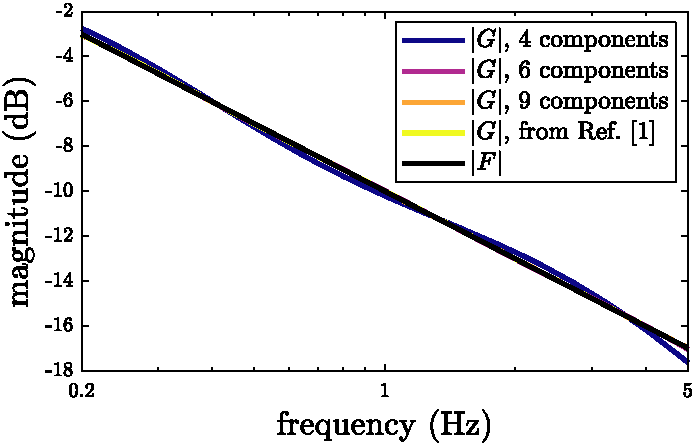
\includegraphics[width=\textwidth]{../ch6/figures/mm1_magnitude.pdf}
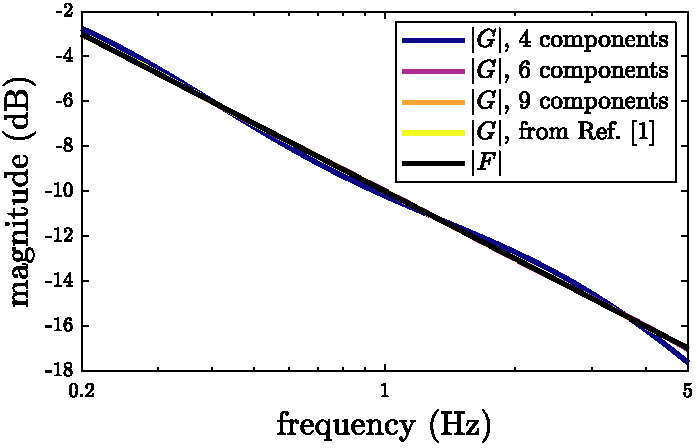
\includegraphics[width=\textwidth]{../ch6/figures/reduced/r_mm1_magnitude}
\caption{Both desired and circuit magnitude response.\label{fig:mm1_magnitude}}
\end{subfigure}%
\begin{subfigure}[t]{0.5\textwidth}
\centering
% 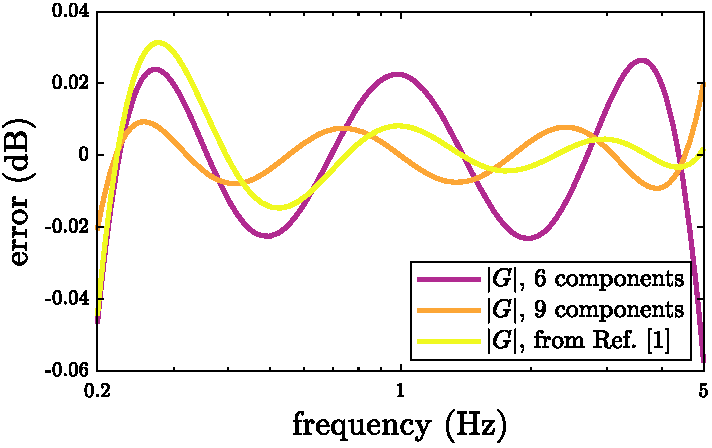
\includegraphics[width=\textwidth]{../ch6/figures/mm1_errors}
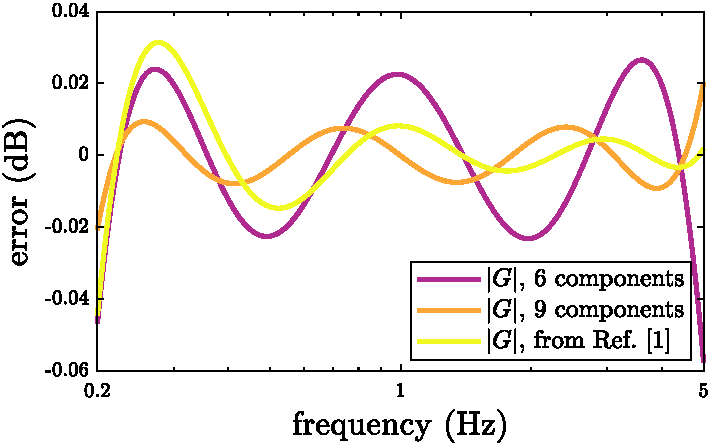
\includegraphics[width=\textwidth]{../ch6/figures/reduced/r_mm1_errors}
\caption{Errors.\label{fig:mm1_errors}}
\end{subfigure}%

\caption[Magnitude and errors over the desired frequency range using select circuits.]{Magnitude and errors over the desired frequency range using select circuits from Fig.~\ref{fig:ch6:ex1:set1}.\label{fig:mm1_magerrors}}

\end{figure}